\documentclass[../main.tex]{subfiles}
\graphicspath{{\subfix{../images/}}}
\begin{document}

%%%%%%%%%%%%%%%%%%%%%%%%%%%%
% \subsubsection{Network Synchronization} \label{time_sync_lan}

The Minion platform employs a hierarchical time synchronization architecture that distributes GPS-disciplined time from the PinPoint receiver to all perception sensors.
% \textcolor{blue}{achieving millisecond-level accuracy for camera observations and microsecond-level synchronization for LiDAR measurements. } 
In this configuration, the GPS clock serves as the master time source, which is distributed over the network via \ac{NTP} for coarse alignment or \ac{PTP} to achieve higher precision.
Together, these layers establish a unified temporal framework supporting reliable cross-modal data fusion and performance evaluation.

The synchronization hierarchy cascades timing information from the PinPoint GPS receiver, through the Atlas computing cluster, to the Jetson Xavier in the camera enclosure, and finally to each Livox Horizon LiDAR unit. This hierarchy is intentionally structured to align with the system’s physical and logical topology:

% PinPoint GPS → Atlas PC (Chrony NTP server) → Jetson Xavier (NTP client, PTP master) → Livox Horizon LiDAR (PTP clients)

At the top of this chain, the PinPoint GPS module provides Coordinated Universal Time (UTC) with sub-microsecond accuracy using the Global Navigation Satellite System (GNSS) signal. This external clock acts as the authoritative reference for the entire vessel, ensuring that all downstream systems inherit a consistent time base independent of internet connectivity.

%%%%%%%%%%%%%%%%%%%%%%%%%%%%
% \subsubsection{Network Time Protocol} \label{NTP}
% \paragraph{NTP}
Within the local area network (LAN), the Chrony \ac{NTP} daemon runs on the primary Atlas computer, which serves as the authoritative time server for all onboard devices. Chrony continuously disciplines the system clock using the GPS reference and corrects for minor drift caused by oscillator instability.

The NVIDIA Jetson AGX Xavier inside the camera enclosure operates as an \ac{NTP} client, synchronizing its system clock with the Atlas PC over the local Ethernet link. The resulting clock alignment achieves approximately 1–10~milliseconds accuracy—sufficient for coordinating 10~Hz camera streams and maintaining consistent ROS timestamps across computing nodes.

The synchronization status is verified at startup by onboard scripts that query Chrony before any video or LiDAR processes begin. This verification ensures that recording never proceeds with unsynchronized clocks. In addition, automated diagnostic checks allow operators to confirm that time distribution remains stable throughout offshore missions, where the GPS link represents the sole external time authority

%%%%%%%%%%%%%%%%%%%%%%%%%%%%
% \subsubsection{Precision Time Protocol} \label{PTP}
% \paragraph{PTP}
While \ac{NTP} provides millisecond-level precision for cameras and computing nodes, LiDAR sensors demand tighter synchronization. Each Livox Horizon operates at 100~Hz with microsecond-timestamped measurements, where even millisecond-level drift would cause measurable spatial distortion during vessel motion. To meet this requirement, the Jetson Xavier distributes the \ac{PTP} signal using the Linux ptp4l service.

In this configuration, the Jetson acts as the \ac{PTP} master clock, broadcasting timing packets over the camera-enclosure network to all three Livox devices, which function as \ac{PTP} slaves. \ac{PTP} uses hardware-timestamped Ethernet packets to measure network delay symmetrically and correct for it in real time, achieving sub-microsecond synchronization between LiDAR units. The Livox Viewer utility confirms synchronization state during system startup, and visual indicators within the GUI report “active 1588 signal” once synchronization is established.

\begin{figure}[htbp]
\centering
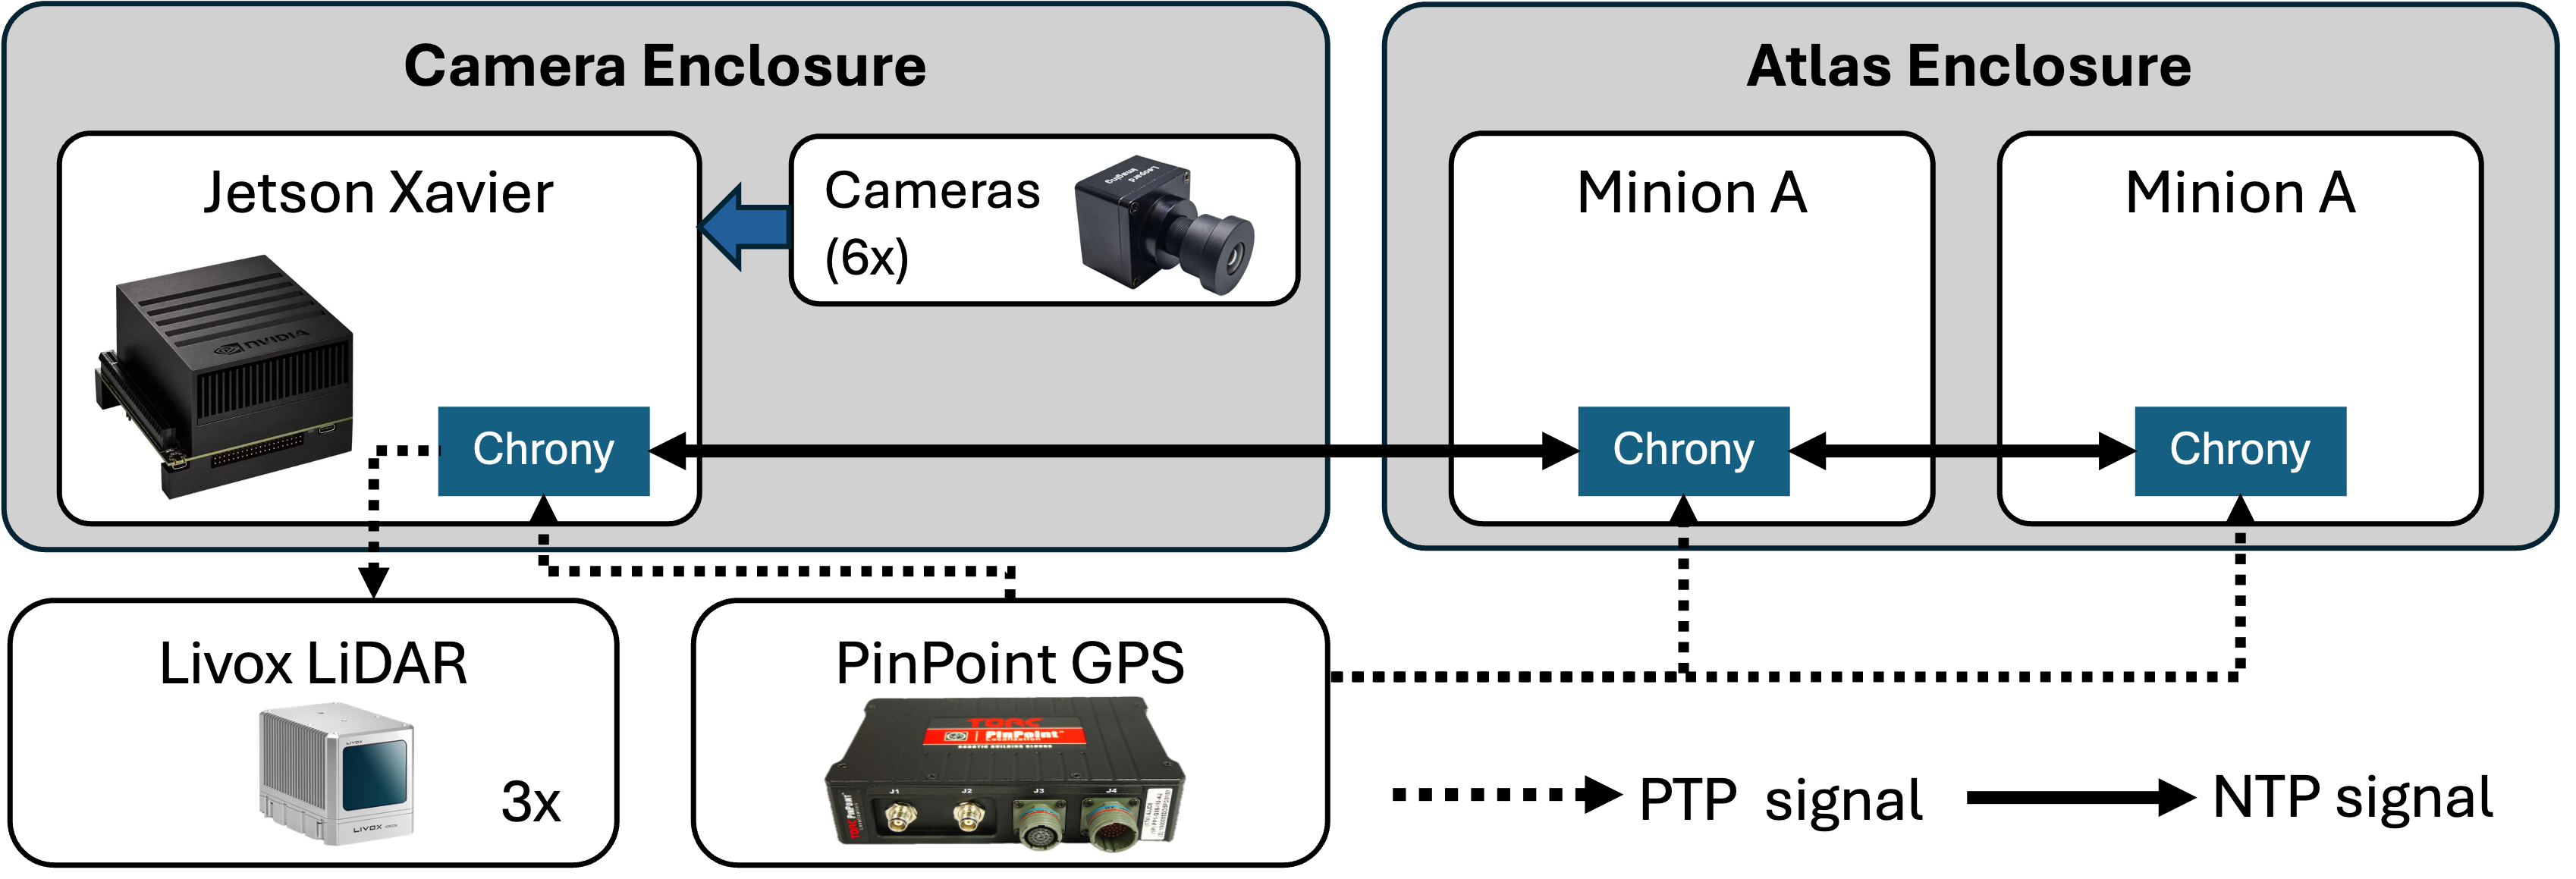
\includegraphics[width=0.8\textwidth]{Images/NTP.png}
\caption{LAN diagram for Minion USV}
\label{fig:network_sync}
\end{figure}

\end{document}